\documentclass[a4paper,11pt]{article}
%\usepackage{ngerman}
\usepackage[utf8]{inputenc}
\usepackage{geometry}
\usepackage{todonotes}
\usepackage{xcolor}
\usepackage{colortbl}
\usepackage{longtable}
\usepackage{array}
\usepackage{eurosym}
%\usepackage{hyperref}
\usepackage[colorlinks=true,breaklinks=true,linkcolor=kolor,urlcolor=kolor,citecolor=kolor]{hyperref}
\usepackage{graphicx}
%\usepackage{psfrag}
\usepackage{fancyhdr}
\usepackage{amssymb}
\usepackage{wrapfig}
%\usepackage[onehalfspacing]{setspace}
\usepackage{framed}
\usepackage{multirow}
%\usepackage{mdframed}
\usepackage{amsmath}
%\usepackage{float}
\usepackage{blindtext}
%\usepackage{printlen}
%\usepackage{multirow}
%\usepackage{rotating}
%\usepackage{math}
\usepackage{titlesec}
\usepackage{etoolbox}
\usepackage{acronym}
\usepackage{pgfplots}
\usepackage{tikz}
\usepackage{pgf-pie}
\usepackage[utf8]{inputenc}
\usepackage{fancyhdr}



\geometry{left=2cm,top=2cm,right=2cm,bottom=2cm}


% define line line spacing
%\renewcommand{\baselinestretch}{1.2}

\renewcommand{\familydefault}{\sfdefault} %font
%\fontfamily{cmr}\selectfont %wie bsc


\definecolor{kolor}{RGB}{0,0,0}
\definecolor{maincol}{RGB}{178,201,225}
\definecolor{darkcol}{RGB}{0,78,155}




\setlength \abovecaptionskip{0pt}   % no spacing above caption

\setlength \parindent{0pt}  % no indent everywhere

% define citation style
\bibliographystyle{unsrt}

% define second level for `itemizing'
\renewcommand{\labelitemii}{-}


\renewcommand{\figurename}{Abbildung}
\renewcommand{\tablename}{Tabelle}
\renewcommand{\refname}{Referenzen}

\titleformat*{\section}{\huge\bfseries}
\titleformat*{\section}{\huge\bfseries}
\titleformat*{\subsection}{\LARGE\bfseries}
\titleformat*{\subsubsection}{\Large\bfseries}
\titleformat*{\paragraph}{\Large\bfseries}
\titleformat*{\subparagraph}{\Large\bfseries}



\makeatletter
\patchcmd{\ttlh@hang}{\parindent\z@}{\parindent\z@\leavevmode}{}{}
\patchcmd{\ttlh@hang}{\noindent}{}{}{}
\patchcmd{\@part}{\markboth{}{}}{\partmark{#1}}{}{} % \part in header
\makeatother
\begin{document}


% Deckblatt

\begin{center}

\thispagestyle{empty}

	\includegraphics[width=8cm]{Images/uni-siegen-logo.png}
	\\
	\vspace*{1cm}
	\Large{Durchgef{\"u}hrt im Rahmen des}\\
	\Huge{\textbf{BMBF-Projekt: ELISE}}\\
	\vspace{1.0cm}
	\Huge{\textbf{Dokumentation der Projektarbeit}}\\
	\vspace{0.3cm}	
	\Large{Entwurf eines kompakten mikrocontrollergest{\"u}tzten Systems zur Emotionserkennung in einer Virtual-Reality-Umgebung}\\
\vspace{0.5cm}	
\Large{\textbf{WiSe 2017/2018 und SoSe 2018}}\\
\vspace{0.6cm}
\end{center}
	
\Large
\noindent
\underline{\textbf{Projektbetreuer:}}\\
\\
\noindent
\textbf{Medizinische Informatik und Mikrosystementwurf}\\
Prof. Dr. rer. nat. Rainer Br{\"u}ck\\
Dr.-Ing. Armin Gr{\"u}newald\\
M.Sc. David Kr{\"o}nert\\
M.Sc. Tanja Eiler\\

\noindent
\textbf{Forschungsgruppe f{\"u}r Mustererkennung}\\
Prof. Dr.-Ing. Marcin Grzegorzek\\
M.Sc. Frédéric Li\\
\vspace*{1.2cm}

\noindent
\underline{\textbf{Projektteilnehmer:}}\\
\\
\noindent
Artur Piet (Sprecher der Projektgruppe)\\
Jonas P{\"o}hler (Stellv. Sprecher der Projektgruppe)\\
Arnaud Eric Toham Waffo\\
Boris Kamdem\\
Kevin Orth\\
Meryem Dural\\
Minas Michail\\


% Inhaltsverzeichnis
\newpage
\renewcommand{\contentsname}{Inhaltsverzeichnis}
\tableofcontents
\clearpage


% Part 0 - Grundlagen


% 1 Allgemeines
\newpage

\section*{Begrifflichkeiten}
\addcontentsline{toc}{section}{Begrifflichkeiten}

\noindent
\todo[inline]{Kurze Beschreibung der verwendeten Begriffe/Abkürzungen}


% 2 Einleitung
\newpage
\section{Einleitung} \label{einleitung-sec}


In der Einleitung sollen zunächst ein paar Grundlegende Voraussetzungen dieser Projektgruppe geklärt werden. So wird in diesem Kapitel zunächst der Hintergrund sowie die Motivation der gesamten Projektgruppe erläutert, danach erfolgt noch eine kurze Projektbeschreibung. Abschließend sollen noch einige Formalien geklärt werden. Dies erfolgt mittels einer Gliederung des kompletten Projekthandbuches, und zuletzt mit einer Auflistung des beigefügten Anhanges.

% Unterkapitel
\subsection{Hintergrund und Motivation} \label{hintergrund-subsec}

\todo[inline,color=green!40]{RfP}

Die Gesellschaft befindet sich seit mehreren Jahren in einem beschleunigten Wandel der das Leben ver{\"a}ndert. 
Dieser Wandel wurde durch die Automation und die Digitalisierung, welche sich beide erg{\"a}nzen verst{\"a}rkt und wird auch als vierte industrielle Revolution bezeichnet, die zu Ver{\"a}nderungen im Alltag als auch in der Wirtschaft gef{\"u}hrt hat. 
Durch die Digitalisierung mussten viele Branchen wie die Musik, Einzelhandel und die Logistik \& Versand Industrie umstrukturieren oder wurden wie zum Beispiel die Schreibmaschinenindustrie vollst{\"a}ndig beseitigt. 
Somit erscheinen t{\"a}glich technologische Innovationen, die im Internet, Fernsehen oder in Zeitschriften ver{\"o}ffentlicht werden. 
Ein Bereich sind die affektiven Technologien. 
Dieser Bereich hat sich als interdisziplin{\"a}res Forschungsfeld etabliert und untersucht die Interaktion zwischen Mensch und Maschine, wobei Emotionen im Mittelpunkt stehen und l{\"a}sst sich in zwei Systeme unterteilen. 
Zu einem die emotionssensitiven Technologien, womit Maschinen verstehen was Menschen f{\"u}hlen und zum anderen die ``Emotional Robotic''- Technologien, die einen Roboter menschen{\"a}hnlicher erscheinen lassen. \\

Um die Forschung im Bereich emotionssensitiven Technologien voranzutreiben wurde ein Forschungsprojekt mit den Namen ``ELISE: Entwicklung von interaktiven und emotionssensitiven Lernsystemen zur Kompetenzerhaltung im Gesch{\"a}ftsprozessmanagement'' ins Leben gerufen (siehe Kapitel \ref{elise-subsec}). \\

Der Lehrstuhl Medizinische Informatik und Mikrosystementwurf entwickelt im Rahmen des Gesamtprojektes ein Sensorsystem, welches die Vital-, Elektroenzephalografie-, Elektrookulografie- und galavanische Hautreaktionwerte aufzeichnet. 
Diese werden dann vom Lehrstuhl f{\"u}r Mustererkennung ausgewertet. 
Die Lerninhalte der Hauptanwendung des ELISE-Projekts werden daraufhin an Emotionen und Gem{\"u}tslagen der Lernenden wie Gl{\"u}ck, Langeweile, Frustration auf Basis von biomedizinischer Daten angepasst, um so den individuellen Erfolg des Lernenden zu erh{\"o}hen. \\

Diese Projektarbeit befasst sich mit dem Entwurf eines kompakten mikrocontrollergest{\"u}tzten Systems zur Emotionserkennung in einer Virtual-Reality-Umgebung. 
Die Projektarbeit baut auf eine vorher am Lehrstuhl geschriebene Master Thesis  auf\cite{msckroenert} und ist eine Zusammenarbeit mit dem Lehrstuhl f{\"u}r Mustererkennung. 
Sie beinhaltet den Aufbau und die Programmierung des Mikrocontrollers, welches zur Kommunikation der verschiedenen biomedizinischen Sensoren dient, die Entwicklung der VR-Umgebung, die Schnittstellen zwischen Hardware und Software und die Speicherung der Rohdaten (Vital-, Elektroenzephalografie-, Elektrookulografie- und galavanische Hautreaktionwerte). 
Diese Rohdaten wurden anhand von Messreihen an 88 Probanden gewonnen und wurden dem Lehrstuhl f{\"u}r Mustererkennung zur Verarbeitung {\"u}bergeben. Die Ergebnisse der Verarbeitung werden auch aufgef{\"u}hrt.  



% Unterkapitel
\subsection{ELISE Projektbeschreibung} \label{elise-subsec}



Elise ist ein Verbundprojekt, welches die Entwicklung eines interaktives und emotionssentives Lernsystem zur Kompetenzentwicklung im Bereich der Gesch{\"a}ftsprozessmanagement plant. 
Hierf{\"u}r kamen f{\"u}nf Partner des Forschungskollegs (FoKoS) der Universit{\"a}t Siegen zusammen – der Lehrstuhl f{\"u}r Wirtschaftsinformatik \& Center for Responsible Innovation \& Design, die Forschungsgruppe Research Group for Patern Recognition, das Institut f{\"u}r Mikrosystemtechnik der Universit{\"a}t Siegen, die Spieleentwickler Limbic Entertainment GmbH und die Softwarehersteller Software AG. 
Zusammen befassen sie sich mit einem interaktiven und emotionssensitiven Lernsystems, im Form eines Spiels, das in einer virtuellen Umgebung erfolgt. 
Zudem befasst sich das Projekt mit der Auswirkung von solcher Systeme hinsichtlich ethischer und gesellschaftlicher Aspekte auf die Akzeptanz potenzieller Nutzerinnen und Nutzer. 
Abbildung \ref{fig-elise} zeigt das vorhaben, welches durch das Projekt Elise verwirklicht werden soll.


\begin{figure}[H] \centering
\includegraphics[width=12cm]{Images/elise_projektbeschreibung.png} 
\vspace{-0.3cm} 
\caption{Grobe {\"u}bersicht des Gesamtprojekts\cite{msckroenert}.}
\label{fig-elise} 
\end{figure}

% Unterkapitel
\subsection{Gliederung dieser Dokumentation} \label{gliederung-subsec}

\todo[inline]{Waiting for Kevin's input.}

% Unterkapitel
\subsection{Anhang}  \label{anhang-subsec}


Der Anhang enthält alle Dateien, die im Rahmen dieser Projektgruppe erstellt wurden, und wird in Form einer beigelegten CD-Rom zur Verfügung gestellt.
Bei diesen Dateien handelt es sich im Wesentlichen um die erstellten Eagle-Dateien (Schaltplan und Layout) die Dateien für den 3 Druck (Maske und Gehäuse) sowie den erstellten Code für den Mikrocontroller und die zu verarbeitende Software.
Zuletzt sind noch alle erstellten Anleitungen, für den Hardwareaufbau und die Versuchsdurchführung enthalten. Eine genaue Beschreibung der in den erwähnten Dateien behandelten Themen erfolgt in den nachfolgenden Kapiteln.
Auf der CD-Rom befinden sich im Ordner Senfemo-Anhang die folgenden Dateien:
\newline
-Eagle-Dateien aller drei Prototypen
\\
-Code für die Prototypen
\\
-Datenblätter der verwendeten Komponenten
\\
-Dateien für den 3D-Druck
\\
-diverse Anleitungen 



% 3 Organisation
\newpage
\section{Organisation} \label{organisation-sec}
\todo[inline]{Verantwortlich: Artur \\}


Diese Projektgruppe des ELISE Projektes wird dem Lehrstuhl Medizinische Informatik \& Mikrosystementwurf und dem Lehrstuhl für Mustererkennung zugeordnet. \\

Die Gruppe wird von Dr.-Ing. Armin Grünewald, David Krönert und Frédéric Li geleitet. 
Innerhalb der Gruppe wurden dazu unabhändig ein Sprecher und ein stellvertretender Sprecher von den Gruppenmitgliedern gewählt. Als Projektgruppensprecher wurde Artur Piet und als Stellvertreter Jonas Pöhler ausgewählt. 
Diese Stellung ist jedoch nicht die eines Leiters mit Entscheidungs- und Weisungsbefugnissen. Die Sprecher sind also auf die Kooperationsbereitschaft der anderen Gruppenmitglieder angewiesen. 
Konkrete Aufgaben der Sprecher waren unter anderen das Verteilen von Verantwortungsbereichen auf alle Mitglieder, die Einführung von regelmäßigen Gruppentreffen um den Überblick über alle Fortschritte zu garantieren und die Übernahme möglichst aller organisatorischer Tätigkeiten (z.B. Messreihen organisieren, Beschaffungsprozesse koordinieren, usw.). \\

Die Laufzeit der Projektgruppe wurde auf etwa 1 Jahr gesetzt, wobei das Kick-Off Meeting am 23.10.2017 stattfand. Der geforderte individuelle Zeitaufwand aller Gruppenmitglieder entspricht der jeweils im Modulhandbuch des Studienganges definierten Leistungspunkte für die Projektarbeit, also 600 Stunden für Jonas Pöhler, Arnaud Eric Toham Waffo, Boris Kamdem, Kevin Orth, Meryem Dural sowie Minas Michail und 270 Stunden für Artur Piet. Es folgt ein Balkendiagramm mit den geforderten Stunden im Verlgeich zum tatsälichem Zeitaufwand. \\

\begin{figure}[h]
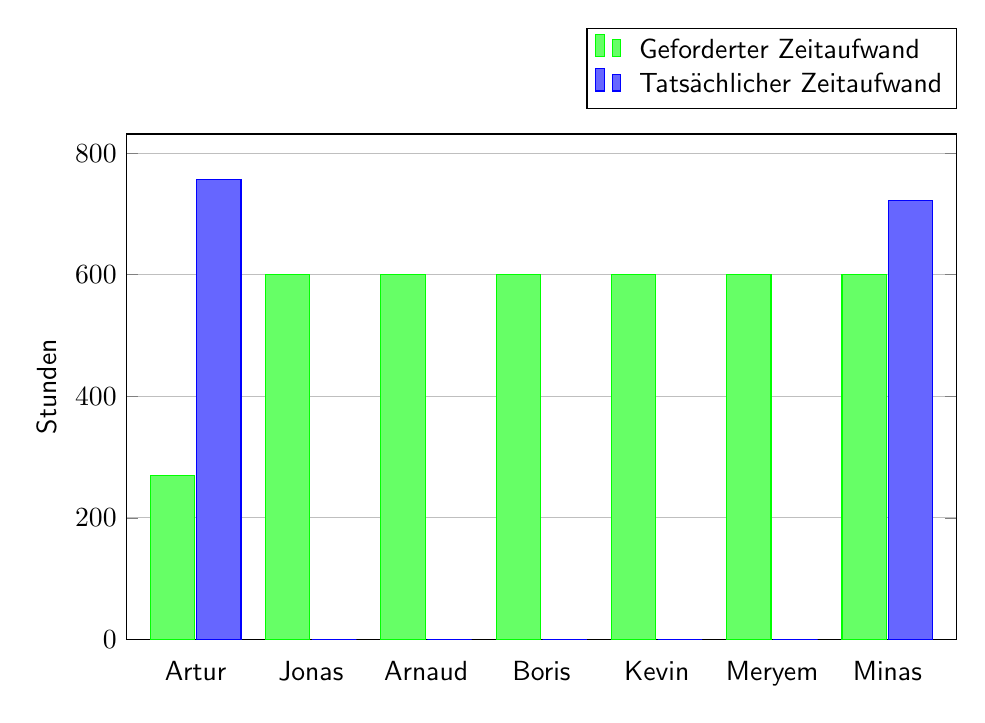
\begin{tikzpicture}
    \begin{axis}[
        width  = \textwidth,
        height = 8cm,
        major x tick style = transparent,
        ybar=2*\pgflinewidth,
        bar width=16pt,
        ymajorgrids = true,
        ylabel = {Stunden},
        symbolic x coords={Artur,Jonas,Arnaud,Boris,Kevin,Meryem,Minas},
        xtick = data,
        scaled y ticks = false,
        enlarge x limits=0.1,
        ymin=0,
        legend cell align=left,
        legend style={
                at={(1,1.05)},
                anchor=south east,
                column sep=1ex
        }
    ]
        \addplot[style={green,fill=green!60,mark=none}]
            coordinates {(Artur, 270) (Jonas,600) (Arnaud,600) (Boris,600) (Kevin,600) (Meryem,600) (Minas,600)};

        \addplot[style={blue,fill=blue!60,mark=none}]
             coordinates {(Artur,756) (Jonas,0) (Arnaud,0) (Boris,0) (Kevin,0) (Meryem,0) (Minas,722)};

        \legend{Geforderter Zeitaufwand,Tatsächlicher Zeitaufwand}
    \end{axis}
\end{tikzpicture} 
%\caption{Stundenaufwand: Vergleich zwischen gefoderten und tatsächlichen Zeitaufwand der Projektgruppenmitglieder.} 
\end{figure} 



\subsection{Verantwortungsbereiche}
Innerhalb der Projektgruppe (PG) war ein Ziel, dass jeder der Mitglieder "Experte" für einen Bereich wird. Damit haben wir die Verantwortung relativ gleichmäßig auf alle aufgeteilt. Dazu muss noch erwähnt werden, dass die Teammitglieder nicht nur ausschließlich die Aufgaben des jeweiligen Verantwortungsbereiches erlegibt habe. Es wurde sich vielmehr gegenseitig immer unterstützt und viel zusammengearbeitet. Die Verantwortungsbereiche haben sich mit der Zeit folgendermaßen aufgeteilt: \\

$ \bullet $ Artur Piet: Mustererkennung, 3D-Konstruktion und Sprecher der PG \\
$ \bullet $ Jonas Pöhler: Hardware, Webanbindung und Stellv. Sprecher der PG \\
$ \bullet $ Arnaud Eric Toham Waffo: Elektrodenauswahl \\
$ \bullet $ Boris Kamdem: Langeweile-Szenario und Fragebogen in VR \\
$ \bullet $ Kevin Orth: Komplette Hardware \\
$ \bullet $ Meryem Dural: Frustations-Szenario in VR \\
$ \bullet $ Minas Michail: Glücks-Szenario in VR \\


\subsection{Gruppentreffen}
Die wöchentliche Gruppentreffen finden immer Donnerstags ab 14:00 Uhr statt und beginnen in der Regel mit einer Update-Runde. Hierbei kommen alle Gruppenteilnehmer der Reihe nach dran und jeder erklärt kurz woran letzte Woche gearbeitet wurde, was die aktuellen Herausfoderungen und Probleme sind und was genau als nächstes geplant ist. Ziel ist es den Austausch und die Kommunikation unter den Teammitgliedern und den Projektleitern zu fördern, damit alle Teilnehmer auf dem selben Wissenstand sind, da einzelnen Aufgaben durchaus großen Einfluß auf Tätigkeiten von anderen Mitgliedern haben können. \\


% 4 Grundlagen
\newpage
\section{Grundlagen} \label{grundlagen-sec}
\todo[inline]{Verantwortlich: Arnaud}



% Unterkapitel
\subsection{Definition von Emotionen} \label{definition-emotionen}


\todo[inline]{Verantwortlich: Arnaud}


Der Begriff ``Emotion'' wird zwar weltweit  (in fast allen Sprachen) und von alle Menschen verwendet (die soziale oder intellektuelle Ebene spielt keine Rolle), ist aber relativ schwer zu definieren. 
Dieses Paradox wurde bereits im folgenden Zitat explizit erwähnt: 
``Everybody knows what an emotion is, until asked to give a definition.''\cite{fehr_russel_1984} von Fehr und Russell, zwei amerikanischer Emotionsforscher (Psychologe). 
Noch überraschender ist die Schwankung in der Definition dieses Begriffs ``Emotion'' im Laufe der Zeit: Allein die englischsprachige Experimentalpsychologie\cite{plamper12} liefert zwischen 1872 und 1980 mehr als 92 verschiedene Definitionen. 
Wir verstehen daher, dass es schwierig wäre, zu versuchen, diese Definition zu formulieren.  
Wie können wir also die Schwierigkeit, eine Definition für einen solchen gemeinsamen Begriff zu finden, erklären? 
Man sollte nicht vergessen werden, dass es sich um einen eher abstrakten Begriff handelt und daher ist die Emotion sehr subjektiv. 
Neben diesem abstrakten Aspekt ist auch anzumerken, dass sich der Begriff der Emotion auch auf viele Bereiche bezieht, die sich ebenso voneinander unterscheiden wie sie variieren: z.B. Literatur, Philosophie, Psychologie usw. 
Neben diesem multidisziplinären Charakter, der die Pluralität der Vorstellungen und Ansätze in jedem Definitionsversuch erklären könnte, ist es auch notwendig, die Variationen von Sprachen, Perioden und sogar Kulturen hinzuzufügen. \\


Es wird uns allein mit dieser Arbeit (und das ist auch nicht von uns erwartet) nicht möglich sein, alle Fragen im Zusammenhang mit der Definition des Begriffs ``Emotion'' zu betrachten, aber wir werden einige konkrete Beispiele vorstellen, um die Komplexität zu veranschaulichen, die sich aus der Suche nach einer Definition von Emotion ergeben kann.  
Die antiken Philosophen\cite{geslin13} waren die ersten, die sich mit Emotionen und ihren Einflüssen auf den Alltag beschäftigen haben. 
Tatsächlich nahmen Stoiker wie Zeno und Plato bereits 370 n. Chr. Emotionen als eine Krankheit der Seele wahr, die für sie ein Hindernis für denjenigen war, der denken wollte. 
Platon geht mit seiner Allegorie von der Höhle tiefer, indem er alles was emotional ist  mit alle vernünftig (verständlich) kontrastiert: das heiß Emotion und Vernunft gehen nicht zusammen. 
Descartes und Aristoteles vervollständigen Platons Beobachtungen, indem sie in die Analyse von Emotionen eine Dualität (positiv und negativ) der Perzeption einbringen. 
Aristoteles glaubt, dass alles, was das Leben auf positive Weise beeinflusst, durch positive Emotionen bedingt ist, und Descartes glaubt, dass Emotionen für unser Überleben unerlässlich sind und dass die Schwäche eines Menschen eng mit der Fähigkeit der Seele verbunden ist, seine Emotionen zu kontrollieren. 
Charles Darwin in seinem präsentierte weitere ebenso faszinierende neue Elemente über Emotionen, ohne den bisherigen Beobachtungen zu widersprechen\cite{darwin1872}. 
Er verallgemeinert die Emotionen für alle Kulturen und fand sogar ähnlichkeit mit Tiere. 
Der Darwin präsentiert  Emotionen  als Körpersignale (oder Reaktionen) auf äußere Handlungen(Externe Ereignisse), begleitet von spezifischen körperlichen Äußerungen wie: Gesichtsausdrücke, Gesten und oft Geräusche, die alle  spezifisch je nach Emotionen sind. \\


So können wir weiterhin andere berühmte wissenschaftliche Namen wie William James\cite{james1884}, Walter Cannon\cite{cannon32}, Stanley Scharter\cite{schachter59} usw. nennen, die zu unterschiedlichen Zeiten und an unterschiedlichen Orten das Thema untersucht haben, mit ebenso relevanten wie unterschiedlichen Schlussfolgerungen, aber die Beobachtung bleibt die gleiche, die Definition bleibt unbeständig.
Neben den Schwierigkeiten, die sich aus den oben genannten unterschiedlichen Wahrnehmungen ergeben, trägt die  tägliche missbräuchliche Verwendung bestimmter Begriffe wie Gefühl, Affekt, Stimmung, Gefühl (um nur einige zu nennen) als Synonym für Emotionen dazu bei  mehr Verwirrung in das Verständnis von Emotionen. Diese Begriffe beziehen sich zwar auf Gemütszustände, sind aber jedoch nicht Synonym von Emotion\cite{plamper12}.
Trotz des fehlenden Konsenses über die Frage der Definition dieses Begriffs gibt es jedoch Elemente, die in allen Definitionsversuchen wiederkehren, nämlich: 

\begin{itemize} \setlength\itemsep{-0.15cm}
  \item das Vorhandensein eines Auslösers;
  \item den psychischen Zustand des Subjekts;
  \item einen bestimmten Körperausdruck;
  \item eine physiologische Reaktion (Herzfrequenz, Atmung,Schwitzen ...);
  \item eine bestimmte Qualität, Intensität und Dauer.
\end{itemize}


Basierend auf den obigen Elementen können wir daher zu dem Schluss kommen, dass wir zwar nicht genau definieren können, was eine Emotion ist, können wir aber jedoch jede davon mit Bestimmte spezifisch  Element in Verbindung setzen: einen Stimulus (der der Auslöser der Emotion ist), eine physiologische und körperliche Reaktion. 
Die Existenz mehrerer verschiedener Emotionen lässt sich gerade wegen der Spezifität dieser Elemente vermuten. 
Im nächsten Teil werden wir versuchen, die verschiedenen Emotionen zu klassifizieren, mit einem besonderen Fokus auf diejenigen, die wir zu induzieren versuchen. \\


Wie bei der Definition von Emotionen gibt es keine einheitliche Klassifizierung von Emotionen. 
Und wie bei den versuchten Definitionen gab es im Laufe der Zeit mehrere vorgeschlagene Klassifikationen, die sich auch im Laufe der Zeit entwickelt haben. 
Diese Mehrheit von klassifikationen ist vermutlich eine Folge des Mangels an Konsens über die Definition selbst. 
Es gibt jedoch zwei Arten von Klassifikationen, die vor allem unterscheidet und durchgesetzt haben: eine dimensionale Klassifikation\cite{geslin13} und eine kategorische Klassifikation\cite{basic_emotions_theories}.




\subsubsection{Kategoriale Klassifikation} \label{kategoriale-klassifikation}

Angetrieben von Charles Darwin, (der auch der erste war, der grundlegende Emotionen identifizierte) diese Vorgehensweise ist die von Emotionsforscher  mit einer evolutionären Ansatz. 
Diese Klassifikation basiert auf der Existenz von eine Reihe von sogenannten Grundemotionen oder primäre Emotionen. 
Diese  Emotionen wäre in einer begrenzten Anzahl und ihre Entwicklung wurde stark von der Evolution  beeinflusst. 
Wie viele Dinge in Bezug auf die Emotionen in allgemein, variiert die Anzahl von Grundemotionen von einem Emotionsforscher zu einem anderen (siehe Tabelle \ref{vergleich-basisemotionen}).


\begin{table}[h] \centering
\begin{tabular}{| p{5cm} | p{11cm} |}
\hline
\textbf{Forscher} & \textbf{Basisemotionen} \\ \hline
Gray (1982) & Furcht, Freude, Ärger \\ \hline
Panksepp (1982) & Furcht, Erwartung, Ärger, Panik \\  \hline
Tomkins (1984) & Furcht, Freude, Ärger, Verzweiflung, Ekel, Überraschung, Interesse, Scham, Zufriedenheit \\  \hline
Plutchik (1980) & Furcht, Freude, Ärger, Traurigkeit, Ekel, Überraschung, Akzeptanz, Erwartung \\  \hline
Arnold (1960) & Furcht, Liebe, Ärger, Traurigkeit, Hass, Hoffnung, Begehren, Mut, Niedergeschlagenheit, Verzweiflung, Widerwille \\  \hline
Oatley \& Johnson-Laird (1987) & Furcht, Glück, Ärger, Traurigkeit, Ekel \\  \hline
Ekman (1982) & Furcht, Freude, Ärger, Traurigkeit, Ekel, Überraschung \\  \hline
Izard (1987) & Furcht, Freude, Ärger, Traurigkeit, Ekel, Überraschung, Interesse,Verachtung \\ \hline
\end{tabular} \caption[Vergleich einige Basisemotions-Theorien]{ Vergleich einige Basisemotions-Theorien\cite{basic_emotions_theories}. } \label{vergleich-basisemotionen}
\end{table}



Obwohl sie sich nicht über die Anzahl der Grundemotionen einig sind, sind sich die Forscher einig über die Existenz komplexerer Emotionen, die die Kombination mehrerer primärer Emotionen wären. 
Basierend auf diesem Ansatz wurden mehrere Theorien entwickelt, um Emotionen darzustellen, von denen eine der bekannte das Plutchik-Modell ist. 
Plutchiks Modell verwendet ein radförmiges Diagramm (siehe Abbildung \ref{plutchik}) und verschiedene Farben, um jede Emotion darzustellen. \\


\begin{figure}[h]
\includegraphics[width=\textwidth]{Images/plutchik.png} 
\vspace{-0.3cm} 
\caption{ Einordnung von Emotion nach Plutchik. }
\label{plutchik} 
\end{figure}


Diese Theorie fundiert sich auf  das acht primäre Emotionen mit einer klare trennung (bzw unterschied) zwischen  primären, sekundären und tertiären Emotionen.
Die verbindet jede primäre Emotion mit spezifischen Motivationssystem und Verhaltendstedenze zur Bewältigung grundlegender adaptiver Probleme (siehe Tabelle \ref{verhalten-funktion}). 


\begin{table}[h] \centering
\begin{tabular}{| p{5.1cm} | p{5.1cm} | p{5.1cm} |}
\hline
\textbf{Subjektiv} & \textbf{Verhalten} & \textbf{Funktion} \\ \hline
Angst, Entsetzen & Rückzug, Flucht  & Schutz \\ \hline
Ärger, Wut & Angriff, Beißen & Zerstörung \\ \hline
Freude, Ekstase & Paarung, Besitz & ergreifen Fortpflanzung \\ \hline
Traurigkeit, Trauer & Weinen, Bitte um Hilfe & Reintegration \\ \hline
Akzeptanz, Anbetung, Vertrauen & Paarbildung, Pflege & Zusammengehörigkeit, Bindung \\ \hline
Ekel, Abscheu & Sich übergeben & Ablehnung, Zurückweisung \\ \hline
Erwartung, Antizipation & Untersuchen & Exploration, Erkundung \\ \hline
Überraschung & Innehalten, Einfrieren & Orientierung \\ \hline
\end{tabular} \caption[ Einige Basisemotionen jeweils mit Verhalten und Funktio ]{ Einige Basisemotionen jeweils mit Verhalten und Funktion\cite{basic_emotions_theories}. } \label{verhalten-funktion}
\end{table}






\subsubsection{Kategoriale Ansatz} \label{kategoriale-ansatz}

Dieser von Wundt\cite{basic_emotions_theories} initiierte Ansatz geht von dem Gedanken aus, dass die emotionale Erfahrung in einem mehrdimensionalen Raum dargestellt werden kann. 
Dieser Zerlegung der emotionale Erfahrung  sollte es ermöglichen, eine genaue Analogie zwischen Emotion und Körperausdruck (Gesichtsausdrücke) herzustellen. 
Dieser Ansatz wurde  daher den Vorteil, dass sie die Tür zu einer möglichen Quantifizierung der emotionalen Erfahrung öffnet. 
Die Idee von Wundt (siehe Abbildung \ref{wundt})  war einer dreidimensionalen Zerlegung(Lust-Unlust, Spannung-Entspannung (Lösung), Beruhigung (Ruhe)-Erregung siehe) der emotionalen Erfahrung. 


\begin{figure}[h]
\includegraphics[width=\textwidth]{Images/wundt.png} 
\vspace{-0.3cm} 
\caption[Einordnung von emotionale Erfahrungsprozess nach Wundt.]{ Einordnung von emotionale Erfahrungsprozess nach Wundt\cite{basic_emotions_theories}. }
\label{wundt} 
\end{figure}


Die Frage nach der Anzahl der Dimensionen, die zur Darstellung der emotionalen Erfahrung notwendig sind, wird jedoch zu mehreren Theorien führen. 
Allerdings schlug Russell\cite{basic_emotions_theories} eine zweidimensionale Darstellung mit sechs primären Emotionen nach Ekam vor (siehe Tabelle \ref{vergleich-basisemotionen}). 
Emotionen werden also dank dieses Modells (siehe Abbildung \ref{russell}) eine horizontale Komponente haben: Valenz (Freude/Verdruss) und eine vertikale Komponente: Erregung (Aktivierung). 


\begin{figure}[h] \centering
\includegraphics[width=12cm]{Images/russell.png} 
\vspace{-0.3cm} 
\caption[Einordnung von emotional Erfahrung nach Russell.]{ Einordnung von emotional Erfahrung nach Russell\cite{basic_emotions_theories}. }
\label{russell} 
\end{figure}


Die Valenz unterscheidet positive Emotionen von negative Emotionen, und die Erregung informiert über körperliche Erregung, die man durch die Anzahl von physiologischen Reaktion feststellen kann. 
Jede Emotion lässt sich als Kombination dieser beiden Parameter darstellen was für eine mathematische auswertung sehr hilfreich sein könnte. 
Dieses Modell hat viel Erfolg gehabt, da er die Darstellung von eine Unendlichkeit von Emotionen erlaubt hat. 
Trotz der unterschiedlichen Anzahl von Dimensionen von verschiedenen Autoren vorgeschlagen, die beiden Dimensionen von Russell (Valenz und Erregung) sind Faktoren die in fast alle Modelle dieses Ansatzes auftreten.





% Unterkapitel
\subsection{Virtual Reality (VR)} \label{grund-vr}


\todo[inline]{Verantwortlich: Arnaud, Boris}

% Unterkapitel
\subsection{Sensoren und biophysiologische Signale zur Emotionserkennung} \label{grund-sensoren-subsec}

\todo[inline]{Verantwortlich: Arnaud, Kevin}

% Unterkapitel
\input{Part-0/4-Grundlagen/3-Sensoren/1-temperatur}

% Unterkapitel
\input{Part-0/4-Grundlagen/3-Sensoren/2-bvp}

% Unterkapitel
\input{Part-0/4-Grundlagen/3-Sensoren/3-spo2}

% Unterkapitel
\input{Part-0/4-Grundlagen/3-Sensoren/4-gsr}

% Unterkapitel
\input{Part-0/4-Grundlagen/3-Sensoren/5-eeg}

% Unterkapitel
\input{Part-0/4-Grundlagen/3-Sensoren/6-eog}

% Unterkapitel
\input{Part-0/4-Grundlagen/3-Sensoren/7-ad-wandler}

% Unterkapitel
\input{Part-0/4-Grundlagen/4-Kommunikation/1-kommunikation}




% Unterkapitel


% Unterkapitel
\input{Part-0/4-Grundlagen/5-Mustererkennung/1-grundlagen-mustererkennung}


% Unterkapitel 
\input{Part-0/4-Grundlagen/5-Mustererkennung/2-emotion-recognition-chain}





% 5 SOA Analyse
\newpage
\section{State-of-the-Art Analyse} \label{soa-sec}
\todo[inline]{Verantwortlich: Jonas}

Die Detektion von Emotionen kann auf unterschiedlichste Art erfolgen. In der Literatur wird neben der Verarbeitung von Biosignalen mittlerweile häufig auf eine Detektion durch Kameras oder durch die Analyse von Sprache gesetzt.(vgl. \cite{}) \\

Die Analyse mittels einer Kamera und der Aufnahme von Gesichtsmimik oder Augenbewegung war in der vorliegenden Arbeit nicht möglich, da die HTC Vive die der Proband während des Experimentes trägt, einen Großteil des Gesichtes und damit die Mimik wie auch die Augen verdeckt. Eine Interaktion mit dem Probanden mittels Sprache war ebenfalls nicht vorgesehen. Dementsprechend blieb nur die Möglichkeit der Detektion von Emotionen mittels Biosignalen. Hierbei wird in der Literatur vor allem die Atemfrequenz, die Hautleitfähigkeit, die elektrische Herzaktivität, die EEG Ableitung und die EOG Ableitung heran gezogen.(vgl. \cite{}) \\

Zur Klassifizierung der Emotionen werden in der Literatur unterschiedliche Techniken verwendet. In neuerer Zeit konzentriert sich die Forschung dabei auf Machine Learning gestützte Ansätze.(vgl. \cite{}) Dabei wird zwischen supervised und unsupervised Modellen unterschieden. Bei den unsupervised Modellen wird insbesondere Sequential Floating Forward Search und k-Nearest Neighbour (k-NN) benutzt. Hierbei handelt es sich um Techniken zur Selektion relevanter Features beziehungsweise zur Klassifizierung von Features durch Gruppenbildung.  Auf der Seite der supervised Modelle sticht vor allem die Nutzung der Support Vecotor Machine (SVM) hervor.(vgl. \cite{}) Hierbei wird wie bei allen supervised Modellen ein Datensatz mit Labels genutzt um das Modell auf die zugrunde liegende Datenmenge zu trainieren. 




% Part 1
\newpage
\part{Erster Prototype}
\addtocontents{toc}{\protect\mbox{}\protect\hrulefill\par}


% 1 Systementwurf
\section{Systementwurf und Konzept} \label{systementwurf-sec}
\todo[inline]{Verantwortlich: Kevin, Jonas}



% Unterkapitel 
\subsection{Anforderungen} \label{anfoderungen-1}

Auf Grundlage der Ziele des Forschungsprojektes ELISE und dem Sichten und Vergleichen von mehr als 30 wissenschaftlichen Veröffentlichungen der letzten 15 Jahre, ergeben sich bestimmte
Anforderungen für den Entwurf eines eigenen Emotionserkennungssystems. Einige wissenschaftliche Veröffentlichungen sind dabei nicht außer Acht zu lassen. Die Foscher von T.
Sharma, S. Bhardwaj und H. B. Maringanti haben in ihrer Veröffentlichung Emotion Estimation
using Physiological Signals versucht, mit Hilfe von GSR, Herzschlagrate,
BVP und der Temperatur Aufschluss über die Emotionen Zorn, Angst, Freude und Traurigkeit
durch Stimulation verschiedener Songs und Videos zu erhalten. Sie erforschten, in
welchen Fällen sich die Körperleitfähigkeit je nach emotionalem Ausdruck unterschiedlich
verhält. H. F. Garcia, A. A. Orozco und M. A. Alvarez versuchten in ihrer Arbeit Dynamic
physiological signal analysis based on Fisher kernels for emotion recognition durch unterschiedliche Klassifizierungsmodelle, die Signale von EEG, EOG, EMG (Elektromyografie),
GSR, Atmung und Temperatur zu analysieren. Dafür wurden 32 Probanden,
die ein 40-minütiges Video mit Musikausschnitten ansahen, aufgezeichnet und ausgewertet.
Durch ein automatisches Regressionsprozess-Modell verbesserten sie dynamische Merkmale
und weitere aufgezeichnete Signale für eine weiterführende Auswertung.
Die Emotionserkennung erfolgte bis vor einigen Jahren in Verbindung mit zusätzlichen Kameras
und Software zur Gesichtsmimik-Erkennung oder Stimmerkennung, nicht jedoch mit
einer reinen Aufnahme von Körpermesswerten. In ELISE sollen insbesondere die lernrelevanten Emotionen Langweile, Frustration, Verwirrung sowie Engagement und Freude erkannt
werden. Die Hardware-Architektur muss auch in diesem Fall wieder das Ziel erfüllen, dass
das Gefühl der Immersion nicht gestört wird. Das heißt, dass das System zur Erkennung von
lernrelevanten Emotionen an möglichst wenigen Stellen am Körper mit zusätzlicher Sensorik
angebracht wird.
Auf Basis der Literaturrecherche, wie in der Bibliographie ausgewiesen, sind folgende Sensoren
zur Aufnahme der lernrelevanten Emotionen ausgewählt worden:

• Gehirnaktivität (EEG)
• Augenbewegung (EOG)
• Blutvolumenpuls (BVP)
• Sauerstoffsättigung im Blut (PPG)
• Hautleitfähigkeit (GSR)
• Körpertemperatur

Da die Sensorwerte zum Mikrocontroller aufgrund ihres räumlichen Abstandes über den
Bus übertragen werden, unterliegen diese Werte den Zeitanforderungen des Datenbusses.
Hier ist zu überprüfen, welches Buskonzept den Zeitanforderungen gewachsen ist.
Um den Aufwand für den Benutzer gering zu halten und die Immersion nicht zu stören,
wird versucht, die Sensorik direkt an der VR-Brille anzubringen. Für die EEG- und
EOG-Sensoren ist dies sowieso notwendig, da diese Messungen lediglich am Kopf stattfinden
können. Zudem soll das Endsystem echtzeitfähig sein, um in der späteren Anwendung
Änderungen und Fluktuationen der Emotionen erkennen zu können und die Schulungen auf
den Lernenden anzupassen. Das Emotionserkennungssystem soll mobil anwendbar sein, da
neuere Versionen der HTC Vive VR-Brille in Zukunft den kabellosen Betrieb unterstützen.
Auch aus diesem Grund ist die Kompaktheit, Energieeffizienz und die Datenübertragung der
einzelnen Sensoren und die Datenübertragung des späteren Gesamtsystems, die ebenfalls
kabellos stattfinden soll, von großem Interesse. Eine mögliche Stelle zur Unterbringung des
Gesamtsystems wäre am Hinterkopf des Probanden, da dort der nötige Platz vorhanden ist
und erforderliche Befestigungsstellen am Kopfband der HTC Vive von Vorteil sind.



% Unterkapitel 
\subsection{Konzept} \label{konzept-1}

Auf Abbildung 1 kann man das Konzept der Architektur erkennen, Dies ist zur besseren Anschauung stark vereinfacht. Hierbei bildet der Mikrocontroller das zentrale Element, welches die einzelnen Sensoren anbindet, steuert und die Messsignale grob zur besseren Auswertung verarbeitet. Zur besseren und möglichst in Echtzeit stattfindeten Verarbeitung werden die Daten an einen externen Rechner weitergeleitet. In der Abbildung findet diese Weiterleitung Drahtlos mittels Bluetooth statt. Es wurden in den verschiedenen Prototypen für diese Zwecke sowohl Bluetooth als auch WLAN verwendet. Für die Teilsysteme EEG und EOG wurden schon einfache Physische Filter auf den Leiterplatten vorgesehen, welche die analogen Signale vorberarbeiten, bevor dies von einem AD-Wandler digitalisiert werden. Da die Elektroden für die EEG und EOG Messung nur am Kopf angebracht werden können, empfiehlt es sich die übrigen festgelegten Werte ebenfalls am Kopf zu messen. Um die Messung für möglichst viele Personen mit unterschiedlichen Kopfformen zu ermöglichen wurde zuerst ein elastisches Kopfband und später eine flexible Maske verwendet. All dies wurde für eine spätere Verwendung mit (unter) einer VR-Brille designet. 





% Unterkapitel
\subsection{Hardwareauswahl} \label{hardwareauswahl-1}



% Unterkapitel 
\input{Part-1/1-Systementwurf/3-Hardwareauswahl/1-auswahlkriterien}

% Unterkapitel 
\input{Part-1/1-Systementwurf/3-Hardwareauswahl/2-festlegung-hardware}



% Unterkapitel
\subsection{Hardwarearchitektur} \label{hardwarearchitektur-1}

In den nächsten Abschnitten werden die verwendeten Sensoren, sowie die dazugehörigen Messschaltungen näher erläutert. Im Rahmen dieser Projektgruppe wurden insgesamt drei Prototypen gefertigt. In einigen Fällen ist der Sensor, und die dazugehörige Schaltung  unverändert geblieben. Bei anderen Sensoren gab es Änderungen. In diesem Fall werden die Sensoren und Schaltungen für jeden Prototypen aufgeführt und erläutert.

Die Auswahl der zur Emotionsbestimmung nötigen Vitaldaten wurde im Rahmen der bereits erwähnten aufbauenden Masterarbeit von David Krönert bestimmt. Dies waren die Körpertemperatur, Sauerstoffsättigung im Blut, Blutvolumenpuls, Hautleitfähigkeit, Gehirnaktivität und die Augenbewegungen. Diese Auswahl von relevanten Vitaldaten wurde im leufe der Projektgruppe nicht mehr geändert. Einzig die genaue Art der Messung hat sich mit den unterschiedlichen Varianten des Messboards geändert. Im folgenden soll deshalb noch eine kurze Erklärung der einzelnen Sensoren erfolgen, und wie sich diese für unterschiedliche Prototypen geändert haben.  

% Unterkapitel
\input{Part-1/1-Systementwurf/4-Hardwarearchitektur/1-gsr}

% Unterkapitel
\input{Part-1/1-Systementwurf/4-Hardwarearchitektur/2-temperatur}

% Unterkapitel 
\input{Part-1/1-Systementwurf/4-Hardwarearchitektur/3-pulsoximeter}

% Unterkapitel 
\input{Part-1/1-Systementwurf/4-Hardwarearchitektur/4-eeg}

% Unterkapitel 
\input{Part-1/1-Systementwurf/4-Hardwarearchitektur/5-eog}

% Unterkapitel
\input{Part-1/1-Systementwurf/4-Hardwarearchitektur/6-datenuebertragung}



% Unterkapitel 
\subsection{Programmierung} \label{programmierung-1}







% Unterkapitel 
\subsection{Aufnahme der {\"u}bertragenen Daten} \label{aufnahme-daten-subsec}

Obwohl mit diesem Prototypen keine Messungen mit Emotionsinduktionen an Probanden durchgeführt wurden, fanden zu Testzwecken natürlich auch hier Datenaufnahmen statt. Diese Daten wurden auch wieder mit SerialPlot erfasst, da hier durch die visuelle Darstellung eine relativ schnelle Beurteilung der Daten möglich war. Anders als im Vorhergehenden Prototypen wurde allerdings nicht mehr auf die Bluetooth-Schnittelle zurückgegriffen. Hier wurden die Daten noch über die eingebaute USB-Schnittstelle übertragen, um mögliche Übertragungsfehler einer drahtlosen Verbindung auszuschließen. Das im ESP32 integrierte WLAN-Modul kam hier also noch nicht zum Einsatz.




% 2 Realisierung
\newpage
\section{Realisierung} \label{realisierung-sec}
\todo[inline]{Verantwortlich: Jonas, Kevin \\
- Next Step: Gliederung erstellen}




% 3 Emotionsinduktion
\newpage
\section{Emotionsinduktion} \label{emotionsinduktion-sec}
\todo[inline]{Verantwortlich: Minas}


Das Kapitel beinhaltet einen Ablauf, die verwendeten Fragebögen und die genutzten Szenarien (Glück, Langeweile, Frustration) der Emotionsinduktion für den ersten Prototypen. 
Kapitel Ablauf beschreibt in welcher Reihenfolge die Szenarien und die Fragebögen aufgerufen wurden. 
In den Kapiteln Fragebogen, Glücks- ,Langeweile- und Frustration-Szenario wird, die Entwicklung und Implementierung erläutert. 
Die Emotioninduktion des ersten Prototypen wurde nicht in einer VR-Umgebung entwickelt. 
Zudem muss angemerkt werden, dass diese Emotionsinduktion für eine Zwischenstudie diente. 
Dadurch wurde der Fokus nicht auf die Implementierung gelegt, welche verschiedene Formate besaß z.B. HTML oder PowerPoint, sondern auf den Inhalt, welches der Proband zu sehen oder zu hören bekam.
Die Emotionsinduktion wurde sowohl in Englisch als auch in Deutsch angeboten.



% Unterkapitel
\subsection{Ablauf} \label{ablauf-subsubsec}


\todo[inline]{Verantwortlich: Minas}


% Unterkapitel 
\subsection{Fragebogen} \label{fragebogen-4}


\todo[inline]{Verantwortlich: Boris}

F{\"u}r dieses Prototyp wurden zwei Arten von Frageb{\"o}gen benutzt. 
Der erste Typ ist sehr {\"a}hnlich mit dem von der zweite Prototyp. Es enth{\"a}lt in dem informativen Teil einen Text, wo es beschrieben wird, wie der Fragebogen ausgef{\"u}llt werden soll. Der andere Teil besteht aus vier Dropdown-Boxen von dreizehn Optionen, die zw{\"o}lf verschiedene Emotionen und einen als null oder neutral geltenden Zustand enthalten. Jede Dropdown-Box entspricht ein Viertelzeit der Szenario. Es soll zwischen die Optionen jeder Dropdown-Box gew{\"a}hlt werden, welche Emotion es am st{\"a}rksten empfindet wird, je nachdem, wann man es f{\"u}hlte, d.h. ob es das erste, zweite, dritte oder letzte Quartal der Zeit des Videos war, um die Emotion zu bew{\"a}ltigen. Unten gibt es ein Button wo man dr{\"u}cken kann, wenn man fertig ist. Allerdings hat man auch die M{\"o}glichkeit seine Wahl zu {\"a}ndern, auch wenn man sich schon im n{\"a}chsten Schritt befindet, indem man in diesem n{\"a}chsten Schritt auf den Zur{\"u}ck-Button dr{\"u}ckt und die gew{\"u}nschten {\"a}nderungen vornimmt. Hierf{\"u}r wird ein Widget Blueprint erstellt, die vier Dropdown-Boxen mit dem gew{\"u}nschten Anzahl an Optionen hinzugef{\"u}gt und die Labels von der unterschiedlichen Optionen der Dropdown-Boxen definiert. Ein Button ``next'' wird auch erstellt um zum n{\"a}chsten Fragebogen zu navigieren. Es wird auch eine zwischen Speicherungsfunktion in ein anderes Skript definiert, die hier aufgerufen wird, um die {\"a}nderung auch nach das dr{\"u}cken von dem ``next'' Button zu Speichern. Dabei wird vier Variablen definiert und die Werte von der gew{\"a}hlten Optionen werden ihnen zugewiesen. \\

(Bild f{\"u}r Fragebogen) \\


Der zweite Typ {\"a}hnelt dem ber{\"u}hmten Modell von James Russels ``circumplex'' \cite{russel_1980}. Es ist ein klassisches Modell mit einer kreisf{\"o}rmigen Struktur, die auf zwei senkrechten Diagonalen ruht. Die vertikale Achse, die die Erregung darstellt, und die horizontale Achse, die die Valenz darstellt. Das Zentrum des Kreises stellt eine neutrale Valenz und ein mittleres Erregungsniveau dar. Andere Emotionen werden auf jeder Ebene des Kreises dargestellt.  Hier wird ein weniger bekanntes Modell verwendet, das ``Self Assessment Manikin'' (SAM). Es besteht aus drei Reihen mit je f{\"u}nf Piktogrammen. Diese Piktogramme stellen den Zustand eines Gesichts nach verschiedenen Arten von Emotionen dar. So repr{\"a}sentiert der erste Bereich die Wertigkeit, der zweite die Erregung und der dritte die Dominanz. Eine Erkl{\"a}rung zu jedem dieser Begriffe ist ebenfalls neben dem Fragebogen enthalten, um die Testpersonen {\"u}ber diese W{\"o}rter aufzukl{\"a}ren.  Bei jeder Avatar und in der Mitte jeder der beiden Avatar befindet sich ein Checkbox.  So muss man f{\"u}r jede Zeile das Checkbox ausw{\"a}hlen, das ihrem emotionalen Zustand am besten entspricht. Man kann nur ein Checkbox pro Zeile markieren und man hat auch die M{\"o}glichkeit wie bei dem ersten Model seine Wahl zu {\"a}ndern. Es kann einfach mit Branch-Bedingungen realisieren werden.  Diese werden auch in eine Widget Blueprint wie f{\"u}r das erste Modell gemacht. Es gibt auch wieder die zwischen Speicherungsfunktion und das Button ``next''. Was neues hier kommt ist das Button ``back'' um wieder zum ersten Fragebogen zu navigieren. 

(Bild f{\"u}r circumplex) \\

% Unterkapitel 
\subsection{Szenarien} \label{szenarien-1}

\todo[inline]{Verantwortlich: Meryem}


Im Folgenden Kapitel werden drei verschiedene Szenarien dargeboten. Die Emotionen Glück, Langweile und Frustration werden hierfür zunächst erläutert. Für jede dieser Emotionen werden Szenarien vorgestellt, bei welchen diese bei den Probanden ausgelöst bzw angeregt werden sollen.


% Unterkapitel 
\input{Part-1/3-Emotionsinduktion/3-Szenarien/1-glueck}

% Unterkapitel 
\input{Part-1/3-Emotionsinduktion/3-Szenarien/2-langeweile}

% Unterkapitel 
\input{Part-1/3-Emotionsinduktion/3-Szenarien/3-frust}


% 4 Messreihe
\newpage


Die zweite Messreihe fand in zwei Räumen des Forschungskolleg Siegens (FoKoS) statt. Die Messreihe wurde in den beiden Wochen vom  14.01.19 bis 25.01.19 statt. Insgesamt wurden Daten von Daten von 97 Personen erhalten. Diese deutliche Steigerung der Teilnehmerzahl im Vergleich zur ersten Messreihe (hier waren es 22 Teilnehmer) wurde durch eine Auszahlung von 10€ erreicht. Bei der vorherigen Messreihe wurde an die Teilnehmer keine Aufwandsentschädigung für die Teilnahme geleistet. Eine genaue Auswertung der Daten folgt in späteren Kapiteln. Von der reinen Durchführung her lässt sich aber sagen, dass es mit nur einer Ausnahme keine Probleme bezüglich VR gab (Schwindel). Die Messungen wurden mit der an vorheriger Stelle schon beschriebenem dritten Prototypen gemacht Abb.1 . Das Messsystem bestand aus dem dritten Prototypen, der in einem extra hierfür gefertigten Gehäuse verbaut wurde. Zusätzlich wurde die in Realisierung beschriebene Maske verwendet. 


% 5 Mustererkennung
\newpage
\section{Mustererkennung} \label{mustererkennung-sec}

\todo[inline]{Verantwortlich: Artur\\
- RfP}

Da an dem ersten Tag der Messreihe noch Probleme bei der Datenversendung bestanden, wurden von den insgesamt 97 getesteten Probenden nur die Daten von nur 88 Personen analysiert.
Mit dem relativ großen Datensatz von 88 Testpersonen, wurde sich entschieden die Mustererkennung vor allem auf DNN-Ansätze mit Verwendung von den Circumplex-Labels zu fokusieren.
Die Gründe dafür waren, dass sich durch dieses Vorgehen die besten Ergebnisse erhofft wurden und ein gewisser Zeitdruck durch das anstehende Projektende.
Die getesteten DNN-Ansätze wurden bereits ausführlich in Kapitel \ref{dnn-1} erklärt.
Weitere Informationen zu den verwendeten Circumplex-Lables können in Kapitel \ref{fragebogen-4} nachgeschlagen werden.

% 6 Ergebnisse
\newpage
\section{Ergebnisse} \label{ergenisse-sec}
\todo[inline]{Verantwortlich: Artur}



% Unterkapitel 
\subsection{Ergebnisse der hand-gefertigten Merkmale} \label{ergebnisse-hc-features-subsec}

Von den insgesamt 22 Probenden wurden bei 7 Elektrodenproblemen festgestellt, weshalb die Qualität der Sensordaten bei diesen 7 Testpersonen angezweifelt wird.
Aus diesem Grund, wurden diese Daten für die Mustererkennung nicht berücksichtigt und der tatsächlich analysierte Datensatz besteht aus insgesamt 15 Probanden.
Zun{\"a}chst wurden die Daten mit einer Normalisierungstechnik vorverarbeitet, die bereits im Kapitel \ref{datenerfassung-0} beschrieben wurde.
Entsprechend der ERC wurde dann den gleitenden Zeitfenster-Segmentierungsansatz (vgl. Kapitel \ref{segmenation-1}) mit den Parametern $T=120$ und $\sigma=30$ verwendet.
Um die optimalen Parameter des SVM-Klassifikators (d.h. Soft-Margin $C$ und Kernelparameter $\gamma$) zu bestimmen, wurde ein Gitter-Suchansatz verwendet.
Es besteht darin, einen Satz m{\"o}glicher Werte f{\"u}r jeden Parameter zu definieren und die Leistungen des Klassifikators f{\"u}r jedes Paar m{\"o}glicher Werte zu testen (d.h. an jedem ``Knoten des Gitters''). \\

\begin{figure}[h]\centering{ \hspace{1cm}
\includegraphics[width=6cm]{Images/grid.png}}
\vspace{0.2cm} \caption[Gitter-Suche]{ Gitter-Suche: Ein definierter Satz m{\"o}glicher Werte f{\"u}r jeden Parameter wird an jedem ``Knoten des Gitters'' getestet. Diese Knoten sind in der Abbildung als rote Punkte markiert. }
\end{figure} 
\vspace{0.5cm}

Die folgenden Werte f{\"u}r $\gamma$ und $C$ wurden getestet:
\begin{center}
${\displaystyle \gamma \in \{0.002; 0.008; 0.03; 0.15; 0.5; 1; 2\}}$ \\
${\displaystyle C \in \{ 0.5; 1; 2; 8; 32; 128; 512 \}}$ \\
\end{center}
\vspace{0.5cm}

Da alle Probanden nicht alle Ziel-Emotionen erlebt bzw. angegeben haben, konnte die Leave-One-Subject-Out Kreuzvalidierung nur bedingt f{\"u}r die Bewertung angewendet werden.
Wir haben daher eine 5-fache Kreuzvalidierung mit entsprechendem F1-Wert verwendet. 

\begin{table}[h]
\center{
\begin{tabular}{|c|c|c|c|c|c|}
\hline
 \textbf{Fold 1} & \textbf{Fold 2} & \textbf{Fold 3} & \textbf{Fold 4} & \textbf{Fold 5} & \textbf{Durchschnitt} \\ \hline
 90.18 & 93.06 & 91.63 & 90.61 & 91.98 & 91.49 \\ \hline
\end{tabular}} \vspace{0.3cm} \caption[Durchschnittlicher F1-Wert]{ Durchschnittlicher F1-Wert in \% f{\"u}r die f{\"u}nf Falten des Datensatzes. }
\end{table}
\vspace{0.5cm}



Die Ergebnisse unserer Experimente zeigen, dass ein solcher Aufbau die Erzielung einer relativ hohen Genauigkeit f{\"u}r die Erkennung der vier Klassen erm{\"o}glicht.
Die Confusion-Matrizen f{\"u}r den handgefertigten Merkmalsansatz unter Verwendung der SVM-Klassifikation ist in der folgenden Tabelle zu finden.

\begin{table}[h]
\center{
\begin{tabular}{|c|c|c|c|c|}
\hline
  & \textbf{Sonstige} & \textbf{Gl{\"u}ck} & \textbf{Frustation} & \textbf{Langeweile} \\ \hline
 \textbf{Sonstige} & \textbf{95.21} & 1.98 & 0.29 & 2.51 \\ \hline
 \textbf{Gl{\"u}ck} & 7.84 & \textbf{90.93} & 0.39 & 0.84 \\ \hline
 \textbf{Frustation} & 8.49 & 2.50 & \textbf{84.14} & 4.87 \\ \hline
 \textbf{Langeweile} & 5.69 & 0.70 & 0.94 & \textbf{92.67} \\ \hline
\end{tabular}} \vspace{0.3cm} \caption[Confusion Matrix]{ Confusion Matrix in \% f{\"u}r die f{\"u}nf Falten des Datensatzes. }
\end{table}


% Unterkapitel 
\subsubsection{Codebook Approach} \label{codebook-approach-subsubsec}







% Unterkapitel
\subsection{Analyse der Ergebnisse} \label{analyse-subsec}


Es sei darauf hingewiesen, dass Lösungen, die auf der Verwendung von Deep Neural Networks (DNNs) zur Extraktion von Merkmalen basieren (z.B. Multi-Layer-Perceptron, Convolutional Neural oder Long-Short-Term-Memory Networks) ebenfalls getestet wurden. Diese Ansätze konnten aber nicht so gute Ergebnisse erzielen, wie die handgefertigten Merkmale. Erkennungsraten für die am wenigsten vertretenen Klassen (insbesondere ``Frustration'') scheinen der Grund für die schwache Performance der DNNs zu sein. Wir gehen davon aus, dass dieses Phänomen durch die relativ geringe Größe unseres Datensatzes verursacht wird. \\

Die schächere Performance des CA hat uns auch überrascht. Der Grund hierfür ist aber sehr wahrscheinlich der selbe wie bei den  DNNs, und zwar der relativ kleine Datensatz. \\

Allgemein deuten die Ergebnisse aber darauf hin, dass unser biomedizinisches Datenerfassungssystem zur Emotionserkennung erfolgreich eingesetzt werden könnte, um ein intelligent adaptives Lernsystems zu verbessern. Zukünftige Arbeiten werden die Verfeinerung des Multisensor-Datenerfassungsgerätes, die Erfassung weiterer und größerer Datensätze für die weitere Mustererkennungsanalyse und die Analyse der Wirksamkeit des Emotionserkennungssystems in einem VR-affektiven Lernkontext beinhalten.







% Part 5
\newpage
\section{Zusammenfassung und Ausblick} \label{ende-sec}
\todo[inline]{Noch nicht zugeordnet}



% Unterkapitel
\subsection{Zusammenfassung} \label{zusammenfassung-subsec}


\todo[inline]{Verantwortlich: Meryem \\
- check comments on last pdf for more info}





% Unterkapitel
\subsection{Fazit} \label{fazit-subsec}









% Unterkapitel
\subsection{Ausblick} \label{ausblick-subsec}


\todo[inline]{Verantwortlich: Minas}








% List of Figures
\newpage 
\renewcommand{\listfigurename}{Abbildungsverzeichnis}
\addcontentsline{toc}{section}{Abbildungsverzeichnis}
\listoffigures


% List of Tables
\newpage
\renewcommand{\listtablename}{Tabellenverzeichnis}
\addcontentsline{toc}{section}{Tabellenverzeichnis}
\listoftables


% Anhang
\newpage
\section*{Anhang}
\addcontentsline{toc}{section}{Anhang}


% Referenzen
\newpage
\bibliographystyle{plain}
\bibliography{References/artur,References/marcin}

\end{document}